\documentclass[a4paper,10pt]{article}
\usepackage[a4paper,top=24mm,bottom=25mm,left=23mm,right=23mm,headheight=15pt]{geometry}
\usepackage{fontspec}
\usepackage{amsmath,amssymb,mathtools}
\usepackage{unicode-math}
\usepackage{fancyhdr}
\usepackage{titlesec}
\usepackage[hidelinks]{hyperref}
\usepackage{microtype}
\usepackage{tikz}
\usetikzlibrary{arrows.meta}

\setmainfont{Times New Roman}
\setmathfont{STIX Two Math}
\setmonofont{Menlo}
\setlength{\parindent}{1.5em}
\setlength{\parskip}{0.2em}
\setlength{\emergencystretch}{3em}
\linespread{1.0}
\allowdisplaybreaks[2]

\titleformat{\section}{\Large\bfseries}{\thesection}{0.7em}{}
\titlespacing*{\section}{0pt}{2.2ex plus 0.5ex}{0.9ex}
\pagestyle{fancy}
\fancyhf{}
\fancyhead[L]{\small Reinforcement Learning \textbar{} Markov Decision Processes}
\fancyhead[R]{\small Selene's Blog}
\fancyfoot[C]{\small\thepage}
\renewcommand{\headrulewidth}{0.4pt}
\hypersetup{pdftitle={Reinforcement Learning | Markov Decision Processes},pdfauthor={Selene}}

\begin{document}
\begin{center}
  {\Large\bfseries Reinforcement Learning \textbar{} Markov Decision Processes\par}
  \vspace{0.5em}
  Selene \quad\textperiodcentered\quad October 13, 2026
\end{center}
\vspace{0.7em}

\section{Markov Processes}

\textbf{The Markov property} states that the future state depends only on the current state, not on the past history.

We can use a state-transition matrix \(P\) to describe the transition probabilities \(p(s_{t+1}=s'\mid s_t=s)\):

\[
P=
\begin{pmatrix}
p(s_1\mid s_1) & p(s_2\mid s_1) & \cdots & p(s_N\mid s_1) \\
p(s_1\mid s_2) & p(s_2\mid s_2) & \cdots & p(s_N\mid s_2) \\
\vdots & \vdots & \ddots & \vdots \\
p(s_1\mid s_N) & p(s_2\mid s_N) & \cdots & p(s_N\mid s_N)
\end{pmatrix}.
\]

\section{Markov Reward Processes}

A Markov reward process adds a reward function to a Markov chain. The reward function gives the expected one-step reward. For an episode with a finite number of steps, the \textbf{return} is the discounted sum of rewards. If the rewards after time \(t\) are \(r_{t+1},r_{t+2},r_{t+3},\ldots\), then the return is

\[
G_t=r_{t+1}+\gamma r_{t+2}+\gamma^2r_{t+3}+\cdots+\gamma^{T-t-1}r_T.
\]

Here, \(T\) is the final time step and \(\gamma\) is the discount factor. When \(0<\gamma<1\), rewards further in the future are discounted more heavily, expressing a preference for rewards received sooner. We define the \textbf{state-value function} as the expected return:

\[
\begin{aligned}
V^t(s)
&=\mathbb{E}[G_t\mid s_t=s] \\
&=\mathbb{E}\left[r_{t+1}+\gamma r_{t+2}+\gamma^2r_{t+3}+\cdots+\gamma^{T-t-1}r_T\mid s_t=s\right].
\end{aligned}
\]

The superscript \(t\) records the dependence on time in a finite-horizon episode.

\section{The Bellman Equation}

\textbf{The Bellman equation} decomposes the value of a state into two parts: the \textbf{expected reward for the next step}, plus the \textbf{discounted expected value of the next state}.

For a time-homogeneous process with an infinite discounted horizon, we write the stationary value function as \(V(s)\):

\[
V(s)=R(s)+\gamma\sum_{s'}p(s'\mid s)V(s').
\]

Here, \(R(s)\) is the expected one-step reward from state \(s\), and \(p(s'\mid s)\) is the probability of moving from \(s\) to \(s'\). The term \(\gamma\sum_{s'}p(s'\mid s)V(s')\) represents the expected discounted return after the first step. For a finite horizon, the corresponding recursion uses \(V^t\) on the left and \(V^{t+1}\) on the right, with \(V^T(s)=0\).

We can write the Bellman equation in matrix form:

\[
\begin{pmatrix}
V(s_1) \\
V(s_2) \\
\vdots \\
V(s_N)
\end{pmatrix}
=
\begin{pmatrix}
R(s_1) \\
R(s_2) \\
\vdots \\
R(s_N)
\end{pmatrix}
+\gamma
\begin{pmatrix}
p(s_1\mid s_1) & p(s_2\mid s_1) & \cdots & p(s_N\mid s_1) \\
p(s_1\mid s_2) & p(s_2\mid s_2) & \cdots & p(s_N\mid s_2) \\
\vdots & \vdots & \ddots & \vdots \\
p(s_1\mid s_N) & p(s_2\mid s_N) & \cdots & p(s_N\mid s_N)
\end{pmatrix}
\begin{pmatrix}
V(s_1) \\
V(s_2) \\
\vdots \\
V(s_N)
\end{pmatrix}.
\]

Combining the Bellman equations for all states gives \(V=R+\gamma PV\). Rearranging yields the \textbf{analytical solution}:

\[
V=(I-\gamma P)^{-1}R.
\]

For a finite state space and \(0\le\gamma<1\), the matrix \(I-\gamma P\) is invertible.

\section{Computing State Values}

\begin{itemize}
  \item \textbf{Monte Carlo:} Starting from state \(s\), sample multiple complete trajectories, compute the return of each trajectory, and average those returns.
  \item \textbf{Dynamic programming:} When the rewards and transition probabilities are known, repeatedly apply the Bellman equation to update the values until they converge. Updating a state's value using the current estimates of its successor states is called \textbf{bootstrapping}.
\end{itemize}

\section{MDPs and MRPs}

In an MRP, the next state is sampled directly from the transition distribution over the state space \(S\). In an MDP, an action comes first: the agent chooses an action \(a\), and the next state is then sampled according to the transition distribution conditioned on both the state and the action. A policy \(\pi(a\mid s)\) describes how the agent chooses actions in state \(s\).

% A self-contained vector reproduction of the diagram in the blog post.
\begin{center}
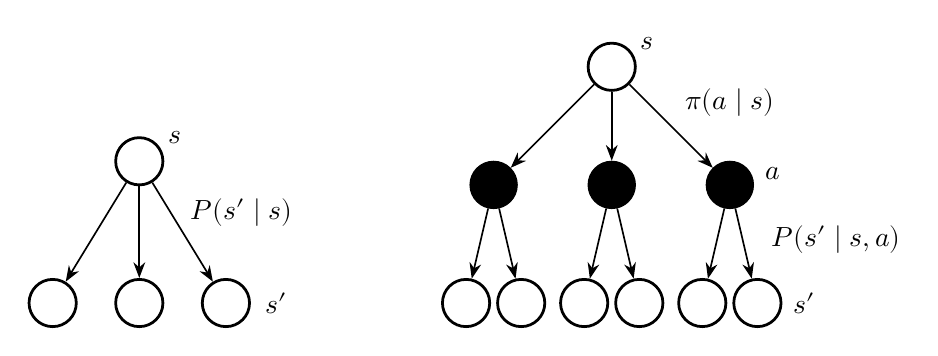
\begin{tikzpicture}[
  state/.style={circle,draw=black,line width=1pt,minimum size=6mm,inner sep=0pt,fill=white},
  action/.style={circle,draw=black,fill=black,minimum size=6mm,inner sep=0pt},
  edge/.style={-{Stealth[length=2mm]},line width=0.6pt}
]
\node[state] (mrp) at (0,1.8) {};
\node at (0.45,2.1) {\(s\)};
\foreach \i/\x in {1/-1.1,2/0,3/1.1} {
  \node[state] (ms\i) at (\x,0) {};
  \draw[edge] (mrp) -- (ms\i);
}
\node at (1.75,0) {\(s'\)};
\node at (1.3,1.15) {\(P(s'\mid s)\)};

\node[state] (mdp) at (6,3) {};
\node at (6.45,3.3) {\(s\)};
\foreach \i/\x in {1/4.5,2/6,3/7.5} {
  \node[action] (a\i) at (\x,1.5) {};
  \draw[edge] (mdp) -- (a\i);
  \node[state] (s\i l) at (\x-0.35,0) {};
  \node[state] (s\i r) at (\x+0.35,0) {};
  \draw[edge] (a\i) -- (s\i l);
  \draw[edge] (a\i) -- (s\i r);
}
\node at (7.5,2.55) {\(\pi(a\mid s)\)};
\node at (8.05,1.65) {\(a\)};
\node at (8.85,0.8) {\(P(s'\mid s,a)\)};
\node at (8.45,0) {\(s'\)};
\end{tikzpicture}
\end{center}

\end{document}
